% ========== Template by IC\M/T Institute of Creative\Media/Technologies =============
% ==========  M. Wagner and K. Blumenstein, N. Thuer 2017 ============= 
% ==========  Based on the LaTeX Thesis Template for the University of Applied Sciences St.Pölten by P. Lechner https://github.com/hrtlacek/ThesisTemplate-FH-StP        ============= 

%----------------------------------------------------------------
% TODO List


%----------------------------------------------------------------

%Dokumentklasse without end dot ;-)
\documentclass[a4paper,twoside,11pt, numbers=noenddot]{scrreprt}
\usepackage[left= 3.5cm,right = 3cm, bottom = 3.5 cm, top = 3 cm]{geometry}
\usepackage[onehalfspacing]{setspace}

% Standard Packages
\usepackage[utf8]{inputenc}

% ============= Settings for the Work =============

\def\workTitle{Isolierte und automatisierte Vernetzung von
Internetdiensten in einer hybriden
Cloud-Infrastruktur}
\def\subTitle{~}
\def\specialization{<Name of Masterclass>}
\def\studentFirstName{Justus}
\def\studentLastName{Mungard}
\def\studentId{931 221}
\def\advisorPreTitle{Dipl.-Inform.}
\def\advisoFirstName{Corina}
\def\advisorLastName{Kopka}
\def\advisorCompanyPreTitle{Dr.}
\def\advisorCompanyFirstName{Roland}
\def\advisorCompanyLastName{Kaltefleiter}
\def\advisorPosTitle{}
\def\assessorPreTitle{}
\def\assessorFirstName{}
\def\assessorLastName{}
\def\assessorPosTitle{}
\def\place{Kiel}
\def\dateDay{20}
\def\dateMonth{05}
\def\dateYear{2021}

\newif\ifuseGermanVersion				    % <== DONT TOUCH THIS!!!
\newif\ifuseMasterInteractiveTechnologies 	% <== CAN'T TOUCH THIS!!! (da da dada)
\newif\ifuseMasterDigitalDesign	            % <== DONT TOUCH THIS!!!
\newif\ifuseMasterDigitalMediaProduction	% <== DONT TOUCH THIS!!!
\newif\ifuseMasterDigitalHealthCare			% <== DONT TOUCH THIS!!!
\newif\ifuseBachelorMediaTechnologiesOne    % <== DONT TOUCH THIS!!!
\newif\ifuseBachelorMediaTechnologiesTwo    % <== DONT TOUCH THIS!!!
\newif\ifuseBachelorSmartEngineeringOne     % <== DONT TOUCH THIS!!!
\newif\ifuseBachelorSmartEngineeringTwo     % <== DONT TOUCH THIS!!!

%***************************************************************************************
% To switch the version please use the comment "%" option :-). After a language change, you have to rebuild the whole project (in Overleaf --> recompile from scratch) 
\useGermanVersiontrue					    % German version
%\useGermanVersionfalse					    % English version
%***************************************************************************************
% To switch between the study programs use the comment option :-) 
% !!!ATTENTION: Only one has to be activated!!!
\useBachelorMediaTechnologiesOnetrue		% Bachelor #1 Media Technology
%\useBachelorMediaTechnologiesTwotrue		% Bachelor #2 Media Technology
%\useMasterInteractiveTechnologiestrue		% Master Interactive Technologies
%\useMasterDigitalDesigntrue		        % Master Digital Design
%\useMasterDigitalMediaProductiontrue		% Master Digital Media Production
%\useMasterDigitalHealthCaretrue			% Master Digital Health Care
% \useBachelorSmartEngineeringOnetrue		% Bachelor #1 Smart Engineering
%\useBachelorSmartEngineeringTwotrue		% Bachelor #2 Smart Engineering
%***************************************************************************************
% Dokumentinformationen
\usepackage[
	pdftitle={\workTitle},
	pdfsubject={},
	pdfauthor={\studentFirstName \studentLastName},
	pdfkeywords={}
	pdftex=true, 
	colorlinks=true,
 	breaklinks=true,
	citecolor=black,
	linkcolor=black,	
	menucolor=black,	
	%urlcolor=black
	urlcolor=magenta
]{hyperref}

\hypersetup{
    bookmarks=true,         % show bookmarks bar?
    unicode=false,          % non-Latin characters in Acrobat’s bookmarks
    pdftoolbar=true,        % show Acrobat’s toolbar?
    pdfmenubar=true,        % show Acrobat’s menu?
    pdffitwindow=false,     % window fit to page when opened
    pdfstartview={FitH},    % fits the width of the page to the window
    pdftitle={My title},    % title
    pdfauthor={Author},     % author
    pdfsubject={Subject},   % subject of the document
    pdfcreator={Creator},   % creator of the document
    pdfproducer={Producer}, % producer of the document
    pdfkeywords={keyword1} {key2} {key3}, % list of keywords
    pdfnewwindow=true,      % links in new window
    colorlinks=false,       % false: boxed links; true: colored links
    linkcolor=black,          % color of internal links (change box color with linkbordercolor)
    citecolor=black,        % color of links to bibliography
    filecolor=black,      % color of file links
    urlcolor=black           % color of external links
}

\usepackage{xurl}
\usepackage{chngcntr}
\usepackage{placeins}
\usepackage{enumitem}
\usepackage[disabled]{todonotes}
\usepackage[toc,acronym]{glossaries}
%https://tex.stackexchange.com/questions/116534/lstlisting-line-wrapping/116572
%https://tex.stackexchange.com/questions/269491/mixing-minted-with-lstlisting
\usepackage[chapter]{minted}
\AtEndEnvironment{listing}{\vspace{-14pt}}

% ============= Packages =============

% Dokumentinformationen
\usepackage[
	pdftitle={\workTitle},
	pdfsubject={},
	pdfauthor={\studentFirstName \studentLastName},
	pdfkeywords={}
	pdftex=true, 
	colorlinks=true,
 	breaklinks=true,
	citecolor=black,
	linkcolor=black,	
	menucolor=black,	
	urlcolor=black
]{hyperref}

\hypersetup{
    bookmarks=true,         % show bookmarks bar?
    unicode=false,          % non-Latin characters in Acrobat’s bookmarks
    pdftoolbar=true,        % show Acrobat’s toolbar?
    pdfmenubar=true,        % show Acrobat’s menu?
    pdffitwindow=false,     % window fit to page when opened
    pdfstartview={FitH},    % fits the width of the page to the window
    pdftitle={My title},    % title
    pdfauthor={Author},     % author
    pdfsubject={Subject},   % subject of the document
    pdfcreator={Creator},   % creator of the document
    pdfproducer={Producer}, % producer of the document
    pdfkeywords={keyword1} {key2} {key3}, % list of keywords
    pdfnewwindow=true,      % links in new window
    colorlinks=false,       % false: boxed links; true: colored links
    linkcolor=black,          % color of internal links (change box color with linkbordercolor)
    citecolor=black,        % color of links to bibliography
    filecolor=black,      % color of file links
    urlcolor=black           % color of external links
}

% Switch the Language
\ifuseGermanVersion
	\usepackage[ngerman]{babel}	% German
\else
	\usepackage[english]{babel} % English
\fi
\usepackage{csquotes}

\usepackage[T1]{fontenc}
%\usepackage{graphicx}
\usepackage{graphicx, subfigure}
%Set path for images
%\graphicspath{{img/}}
\usepackage{fancyhdr}
\usepackage{lmodern}
\usepackage{color}
\usepackage{transparent}

% Zitierstil
% Citation style
%\usepackage[comma,authoryear]{natbib}
%\usepackage{natbib}

%\usepackage[backend=biber, style=apa, citestyle=authoryear, sorting=nyt]{biblatex}

%\ifuseGermanVersion
%    \DeclareLanguageMapping{ngerman}{ngerman-apa}
%\else
%    \DeclareLanguageMapping{english}{english-apa}
%\fi

\usepackage[nottoc]{tocbibind}
%\addbibresource{biblatex.bib}

% zusätzliche Schriftzeichen der American Mathematical Society
\usepackage{amsfonts}
\usepackage{mathtools}

\usepackage[export]{adjustbox}

% BlockDiagram Drawing Package
% ---tikz
\usepackage{tikz}
\usetikzlibrary{positioning}
\usepackage{pgfplots}
\pgfplotsset{compat=1.10}
\usepackage{textcomp}

%====================================================
% Code Block Style Definition
\documentclass{article}
\usepackage[utf8]{inputenc}

\usepackage{listings}
\usepackage{xcolor}

\definecolor{codegreen}{rgb}{0,0.6,0}
\definecolor{codegray}{rgb}{0.5,0.5,0.5}
\definecolor{codepurple}{rgb}{0.58,0,0.82}
\definecolor{backcolour}{rgb}{0.95,0.95,0.92}

\lstdefinestyle{mystyle}{
    backgroundcolor=\color{backcolour},   
    commentstyle=\color{codegreen},
    keywordstyle=\color{magenta},
    numberstyle=\tiny\color{codegray},
    stringstyle=\color{codepurple},
    basicstyle=\ttfamily\footnotesize,
    breakatwhitespace=false,         
    breaklines=true,                 
    captionpos=b,                    
    keepspaces=true,                 
    numbers=left,                    
    numbersep=5pt,                  
    showspaces=false,                
    showstringspaces=false,
    showtabs=false,                  
    tabsize=2
}

\lstset{style=mystyle}
%====================================================

%Package for using the [H] option on graphics to force them into place
\usepackage{float}

%iPython packages:
%\usepackage{graphicx} % Used to insert images
\usepackage{adjustbox} % Used to constrain images to a maximum size 
\usepackage{color} % Allow colors to be defined
\usepackage{enumerate} % Needed for markdown enumerations to work
\usepackage{geometry} % Used to adjust the document margins
\usepackage{amsmath} % Equations
\usepackage{amssymb} % Equations
%\usepackage[mathletters]{ucs} % Extended unicode (utf-8) support
% \usepackage[utf8x]{inputenc} % Allow utf-8 characters in the tex document
\usepackage{fancyvrb} % verbatim replacement that allows latex
\usepackage{grffile} % extends the file name processing of package graphics 
                         % to support a larger range 
    % The hyperref package gives us a pdf with properly built
    % internal navigation ('pdf bookmarks' for the table of contents,
    % internal cross-reference links, web links for URLs, etc.)
\usepackage{hyperref}
\usepackage{longtable} % longtable support required by pandoc >1.10

% embedding of audio/video files etc.
% \usepackage{attachfile}
% \usepackage{movie15}
% \usepackage{media9}
% \usepackage{menukeys}

\usepackage[labelfont=it, labelsep=period, format=plain,justification=raggedright, singlelinecheck=false]{caption}
\captionsetup[figure]{justification=centering}
\definecolor{light-gray}{gray}{0.85}

% Switch between German and English based on the Settingx.tex. file
\usepackage{ifthen}

%\captionsetup[listing]{
%  labelsep = newline,
%  textfont = sc, 
%  name = LISTING, 
%  justification=justified,
%  singlelinecheck=false,%%%%%%% a single line is centered by default
%  labelsep=colon,%%%%%%
%  skip = \medskipamount}

% =============== BlockDiagram Drawing Config
\usetikzlibrary{shapes,arrows}

% Definition of blocks:
\tikzset{%
  block/.style    = {draw, thick, rectangle, minimum height = 3em,
    minimum width = 3em},
  sum/.style      = {draw, circle, node distance = 2cm}, % Adder
  input/.style    = {coordinate}, % Input
  output/.style   = {coordinate}, % Output
  mult/.style	  = {draw, isosceles triangle, minimum height=1cm, minimum width =1cm}
}
%mult/.style	  = {isosceles triangle, sharp corners, anchor=center, xshift=-4mm, minimum height=1.5cm, minimum width =0.05cm}
%isosceles triangle, fill=gray!25, minimum width=1.5cm

% Defining string as labels of certain blocks.
\newcommand{\suma}{\Large$+$}
\newcommand{\inte}{$\displaystyle \int$}
\newcommand{\derv}{\huge$\frac{d}{dt}$}
\newcommand{\conv}{\huge$\ast$}

% ============================================

% -- Settings für Code abbildungen
\usepackage{listings,lstautogobble}
\lstset{backgroundcolor=\color{light-gray},frame=single, framerule=0pt, showspaces=false, showtabs=false, numbers=left, numbersep=5pt, breaklines=false, autogobble=true, language=C++}

% Setze arial font
\usepackage[scaled]{helvet}
\renewcommand*{\familydefault}{\sfdefault}

% FH-grünBlau
\definecolor{FH}{rgb}{0.10, 0.57, 0.68}
% FH-grünBlau 2
\definecolor{FH2}{rgb}{0.0392, 0.666, 0.549}

% nicht einrücken nach Absatz
\setlength{\parindent}{0cm}

% Paragraph-Abstand
\setlength{\parskip}{0.3cm}

% ============= Kopf- und Fußzeile =============

%\renewcommand{\headrulewidth}{0.4pt}
%\renewcommand{\footrulewidth}{0pt}

\renewcommand{\chaptermark}[1]{\markboth{\thechapter~ #1}{}}

\fancypagestyle{icmt-fancy}{%
  \fancyhf{}% Clear header and footer
  \fancyhead[L]{\leftmark}
  \fancyfoot[R]{\thepage}% Custom footer
  \renewcommand{\headrulewidth}{0.4pt}% Line at the header visible
  \renewcommand{\footrulewidth}{0.0pt}% Line at the footer visible
}

% Redefine the plain page style
\fancypagestyle{plain}{%
  \fancyhf{}%
  \fancyfoot[R]{\thepage}%
  \renewcommand{\headrulewidth}{0pt}% Line at the header invisible
  \renewcommand{\footrulewidth}{0.0pt}% Line at the footer visible
}

% ============= Package Einstellungen & Sonstiges ============= 


%Besondere Trennungen
\hyphenation{De-zi-mal-tren-nung St-rei-fen-licht-scan-nern}

%römische Aufzählungen mit \RM{Zahl}
\newcommand{\RM}[1]{\MakeUppercase{\romannumeral #1}}


% ============= Dokumentbeginn =============

\begin{document}

% Select the right main page ;-)
\ifuseGermanVersion
	
% setup page dimensions for titlepage
\newgeometry{left=2.4cm,right=2.4cm,bottom=2.5cm,top=2cm}

% force baselineskip and parindent
%\newlength{\tmpbaselineskip}
%\setlength{\tmpbaselineskip}{\baselineskip}
%\setlength{\baselineskip}{13.6pt}
%\newlength{\tmpparindent}
%\setlength{\tmpparindent}{\parindent}
%\setlength{\parindent}{17pt}

% first titlepage
\pagestyle{empty}

\begin{figure}[H]
\vspace*{-2.5cm}
\hspace*{2.5cm}

\includegraphics[keepaspectratio, width=1.31\textwidth, right]{TemplateElements/Fachhochschule_Kiel-logo.svg.png}
\end{figure}



\begin{center}

\vspace{1cm}

\begin{minipage}[t][5cm][s]{\textwidth}%
\centering
\Huge{{\color{FH2}{\fontsize{24}{30} \selectfont \workTitle\\}}}
\vspace{0.5cm}
\LARGE{{\color{FH2}{\fontsize{16}{24} \selectfont \subTitle\\}}}
\end{minipage}

\vspace{1cm}


\ifnum\ifuseBachelorMediaTechnologiesOne 1
\else\ifuseBachelorSmartEngineeringOne 1
\else0
\fi\fi
=1 
   	\LARGE{Bachelorarbeit}
\else
	\ifnum\ifuseBachelorMediaTechnologiesTwo 2
	\else\ifuseBachelorSmartEngineeringTwo 2
\else0
\fi\fi
=2
	\LARGE{Bachelorarbeit}
\else
	\ifuseMasterInteractiveTechnologies
		\LARGE{Masterarbeit}
	\else
	\ifuseMasterDigitalDesign
		\LARGE{Masterarbeit}
	\else
    \ifuseMasterDigitalMediaProduction
		\LARGE{Masterarbeit}
	\else
	\ifuseMasterDigitalHealthCare
		\LARGE{Masterarbeit}
    \else
        \LARGE{YOU HAVE TO CHOOSE THE PROGRAM TYPE IN THE SETTINGS!!!}
    \fi\fi\fi\fi
\fi\fi

% \ifuseBachelorMediaTechnologiesOne
% 	\LARGE{Research Paper}
% \else
% 	\ifuseBachelorSmartEngineeringOne
%     	\LARGE{Research Paper}
% \else
% 	\ifuseBachelorMediaTechnologiesTwo
% 		\LARGE{Bachelorarbeit}
% \else
% 	\ifuseMasterDigitalMediaTechnologies
% 		\LARGE{Masterarbeit}
% \else
% 	\ifuseMasterDigitalHealthCare
% 		\LARGE{Masterarbeit}
%     \else
%         \LARGE{YOU HAVE TO CHOOSE THE PROGRAM TYPE IN THE SETTINGS!!!}
%   	\fi
% \fi
% \fi
% \fi
% \fi




\vspace{1.3cm}
\ifuseBachelorMediaTechnologiesOne
	\fontsize{11pt}{15pt}\selectfont Bachelor Informationstechnologie\\
	Fachbereich Informatik und Elektrotechnik\\
Fachhochschule Kiel University of Applied Sciences\\  
\else
	\ifuseBachelorMediaTechnologiesTwo
		\fontsize{11pt}{15pt}\selectfont Bachelor-Studiengang \\
Fachhochschule Kiel\\  
\else
	\ifuseBachelorSmartEngineeringOne
    	\fontsize{11pt}{15pt}\selectfont Bachelor-Studiengang Smart Engineering\\
Fachhochschule Kiel\\ 
\else
	\ifuseMasterInteractiveTechnologies
		\fontsize{11pt}{15pt}\selectfont Ausgeführt zum Zweck der Erlangung des akademischen Grades\\
		\textbf{Dipl.-Ing. für technisch-wissenschaftliche Berufe}
\else
	\ifuseMasterDigitalDesign
		\fontsize{11pt}{15pt}\selectfont Ausgeführt zum Zweck der Erlangung des akademischen Grades\\
		\textbf{Dipl.-Ing. für technisch-wissenschaftliche Berufe}	
\else
    \ifuseMasterDigitalMediaProduction
		\fontsize{11pt}{15pt}\selectfont Ausgeführt zum Zweck der Erlangung des akademischen Grades\\
		\textbf{Dipl.-Ing. für technisch-wissenschaftliche Berufe}	
\else
	\ifuseMasterDigitalHealthCare
    	\fontsize{11pt}{15pt}\selectfont Ausgeführt zum Zweck der Erlangung des akademischen Grades\\
		\textbf{Master of Science in Engineering (MSc)}
    \else
        \LARGE{YOU HAVE TO CHOOSE THE PROGRAM TYPE IN THE SETTINGS!!!}
\fi\fi\fi\fi\fi\fi\fi

\vspace{4mm}

\ifuseMasterInteractiveTechnologies
	am Masterstudiengang Interactive Technologies an der\\ 
Fachhochschule St. Pölten, Masterklasse \specialization
\else
    \ifuseMasterDigitalDesign
	am Masterstudiengang Digital Design an der\\ 
Fachhochschule St. Pölten, Masterklasse \specialization
\else
    \ifuseMasterDigitalMediaProduction
	am Masterstudiengang Digital Media Production an der\\ 
Fachhochschule St. Pölten, Masterklasse \specialization
\else
	\ifuseMasterDigitalHealthCare
		am Masterstudiengang Digital Healthcare\\ 
an der Fachhochschule St. Pölten
    \else
        
  	\fi\fi\fi\fi

\vspace{1cm}
\ifuseBachelorMediaTechnologiesOne
	Vorgelegt von:
    
\else
	Ausgeführt von:\\ 
\fi
\fontsize{15pt}{15pt}\selectfont
\textbf{\studentFirstName\ \studentLastName} \\
\fontsize{11pt}{15pt}\selectfont
\studentId

\vspace{1cm}
\ifuseBachelorMediaTechnologiesOne
	\begin{tabular}{lll}
    Erstprüferin: & & \advisorPreTitle\ \advisoFirstName\ 		\advisorLastName\\
    Zweitprüfer: & & \advisorCompanyPreTitle\ \advisorCompanyFirstName\ \advisorCompanyLastName\\
    \end{tabular}
\else
	\ifuseBachelorMediaTechnologiesTwo
		\begin{tabular}{lll}
        Betreuer/in: & & \advisorPreTitle\ \advisoFirstName\ \advisorLastName, \advisorPosTitle\\
        %Zweitbegutachter/in: & & [Titel Vorname Zuname]
		\end{tabular}
\else
\begin{tabular}{lll}
Betreuer/in: & \advisorPreTitle\ \advisoFirstName\ \advisorLastName, \advisorPosTitle\\
Zweitbetreuer/in: & \assessorPreTitle\ \assessorFirstName\ \assessorLastName, \assessorPosTitle\\
\end{tabular}

\fi
\fi

\vspace{1cm}


\large{\place, \dateDay.\dateMonth.\dateYear}


\end{center}

\restoregeometry
\else
	
% setup page dimensions for titlepage
\newgeometry{left=2.4cm,right=2.4cm,bottom=2.5cm,top=2cm}

% force baselineskip and parindent
%\newlength{\tmpbaselineskip}
%\setlength{\tmpbaselineskip}{\baselineskip}
%\setlength{\baselineskip}{13.6pt}
%\newlength{\tmpparindent}
%\setlength{\tmpparindent}{\parindent}
%\setlength{\parindent}{17pt}

% first titlepage
\pagestyle{empty}

\begin{figure}[H]
\vspace*{-2.5cm}
\hspace*{2.5cm}
\includegraphics[keepaspectratio, width=1.4\textwidth, right]{TemplateElements/fhLogo3.png}
\end{figure}



\begin{center}

\vspace{1cm}

\begin{minipage}[t][5cm][s]{\textwidth}%
\centering
\Huge{{\color{FH2}{\fontsize{24}{30} \selectfont \workTitle\\}}}
\vspace{0.5cm}
\LARGE{{\color{FH2}{\fontsize{16}{24} \selectfont \subTitle\\}}}
\end{minipage}

\vspace{1cm}

\ifuseBachelorMediaTechnologiesOne
	\LARGE{Research Paper}
\else
	\ifuseBachelorMediaTechnologiesTwo
		\LARGE{Bachelor Thesis}
\else
	\ifuseMasterInteractiveTechnologies
		\LARGE{Master Thesis}
\else
	\ifuseMasterDigitalDesign
		\LARGE{Master Thesis}
\else
    \ifuseMasterDigitalMediaProduction
		\LARGE{Master Thesis}
\else
	\ifuseMasterDigitalHealthCare
		\LARGE{Master Thesis}
    \else
        \LARGE{YOU HAVE TO CHOOSE THE PROGRAM TYPE IN THE SETTINGS!!!}
  	\fi
\fi
\fi
\fi\fi\fi
  
\vspace{1.3cm}
\ifuseBachelorMediaTechnologiesOne
	\fontsize{11pt}{15pt}\selectfont Bachelor Course on Media Technology\\
at St. Pölten University of Applied Sciences\\  
\else
	\ifuseBachelorMediaTechnologiesTwo
		\fontsize{11pt}{15pt}\selectfont Bachelor Course on Media Technology\\
at St. Pölten University of Applied Sciences\\  
\else
	\ifuseMasterInteractiveTechnologies
		\fontsize{11pt}{15pt}\selectfont For attainment of the academic degree of\\
		\textbf{Dipl.-Ing. für technisch-wissenschaftliche Berufe}
\else
    \ifuseMasterDigitalDesign
		\fontsize{11pt}{15pt}\selectfont For attainment of the academic degree of\\
		\textbf{Dipl.-Ing. für technisch-wissenschaftliche Berufe}
\else
    \ifuseMasterDigitalMediaProduction
		\fontsize{11pt}{15pt}\selectfont For attainment of the academic degree of\\
		\textbf{Dipl.-Ing. für technisch-wissenschaftliche Berufe}
\else
	\ifuseMasterDigitalHealthCare
    	\fontsize{11pt}{15pt}\selectfont For attainment of the academic degree of\\
		\textbf{Master of Science in Engineering (MSc)}
    \else
        \LARGE{YOU HAVE TO CHOOSE THE PROGRAM TYPE IN THE SETTINGS!!!}
  	\fi
\fi
\fi
\fi\fi\fi

\vspace{4mm}
 
\ifuseMasterInteractiveTechnologies
	in the Masters Course Interactive Technologies at St. Pölten\\ 
University of Applied Sciences, Masterclass \specialization
\else
    \ifuseMasterDigitalDesign
	in the Masters Course Digital Design at St. Pölten\\ 
University of Applied Sciences, Masterclass \specialization
\else
    \ifuseMasterDigitalMediaProduction
	in the Masters Course Digital Media Production at St. Pölten\\ 
University of Applied Sciences, Masterclass \specialization
\else
	\ifuseMasterDigitalHealthCare
		in the Masters Course Digital Healthcare\\ 
at St. Pölten University of Applied Sciences
    \else
  	\fi
\fi\fi\fi





\vspace{1cm}

Submitted by:\\ 
\fontsize{15pt}{15pt}\selectfont
\textbf{\studentFirstName\ \studentLastName} \\
\fontsize{11pt}{15pt}\selectfont
\studentId

\vspace{1cm}
\ifuseBachelorMediaTechnologiesOne
	\begin{tabular}{lll}
    Advisor: & & \advisorPreTitle\ \advisoFirstName\ 		\advisorLastName, \advisorPosTitle\\
    %Zweitbegutachter/in: & & [Titel Vorname Zuname]
    \end{tabular}
\else
	\ifuseBachelorMediaTechnologiesTwo
		\begin{tabular}{lll}
        Advisor: & & \advisorPreTitle\ \advisoFirstName\ \advisorLastName, \advisorPosTitle\\
        %Zweitbegutachter/in: & & [Titel Vorname Zuname]
		\end{tabular}
\else
  \begin{tabular}{lll}
  Advisor: & \advisorPreTitle\ \advisoFirstName\ \advisorLastName, \advisorPosTitle\\
  Second Advisor: & \assessorPreTitle\ \assessorFirstName\ \assessorLastName, \assessorPosTitle\\
  \end{tabular}

\fi
\fi

\vspace{1cm}


\large{\place, \dateDay.\dateMonth.\dateYear}


\end{center}

\restoregeometry
\fi

% \part im Inhaltsverzeichnis nicht nummerieren
\makeatletter
\let\partbackup\l@part
\renewcommand*\l@part[2]{\partbackup{#1}{}}

%Seitennummerierung neu beginnen, Zahlen [arabic], röm.Zahlen [roman,Roman], Buchstaben [alph,Alph]
\pagenumbering{Roman}

\newpage

\chapter*{Eidesstattliche Erklärung}
\label{ch:erklaerung}

\begin{flushleft}
Ich versichere mit meiner eigenhändigen Unterschrift, dass ich die vorliegende Abschlussarbeit selbständig und ohne unzulässige, fremde Hilfe angefertigt habe und dass ich alle von anderen Autor*innen wörtlich übernommenen Stellen wie auch die an die Gedankengänge und Strukturen anderer Autor*innen eng angelehnten Ausführungen meiner Arbeit besonders gekennzeichnet und die entsprechenden Quellen angegeben habe.
\end{flushleft}

\begin{flushleft}
Weiterhin versichere ich, dass die vorliegende Abschlussarbeit noch keiner Prüfungsbehörde vorgelegen hat.
\end{flushleft}

Ort: \hrulefill\enspace Datum:	\hrulefill\enspace Unterschrift: \hrulefill
\\[3.5cm]
\newpage

%Inhaltsverzeichnis
\pagestyle{plain}
\tableofcontents

\newpage
%Seitennummerierung neu beginnen, Zahlen [arabic], röm.Zahlen [roman,Roman], Buchstaben [alph,Alph]
\pagenumbering{arabic}

% pagestyle für gesamtes Dokument aktivieren
\pagestyle{icmt-fancy}
\newpage


%Alle Codebeispiele finden sich im Github
% \include{Chapters/02_Recherche_und_Auswahl_der_Komponenten}
\chapter{Definition der Use-Cases} \label{Umsetzung der Use-Cases und Evaluation}

\section{Kundenumfeld und typische Bedürfnisse} \label{Kundenumfeld und typische Bedürfnisse}

Wie bereits eingangs erwähnt, sollen die Use-Cases typische Bedürfnisse von Unternehmen aus dem kleinen und mittelständischen Bereich widerspiegeln (KMU). So ist die Grundannahme, dass der Kunde bereits Rechenressourcen in Selbstverwaltung (\glqq Private Cloud\grqq{}) besitzt. Weiterhin hat die Integration von Public Cloud-Diensten noch gar nicht oder nur oberflächlich stattgefunden: Es wurden ein paar Maschinen hochgefahren und bestimmte Internetdienste installiert. Über eine tiefergehende Koppelung mit bestehenden Diensten und Systemen hat der Kunde bisher keine Überlegungen angestellt. %Eine private Adressierung der Systeme ist noch nicht möglich, die Maschinen werden über die öffentlichen IPs aus dem Internet erreicht. Die Firma besitzt eine private Cloud
%ToDo: Genauer beschreiben, was beim Kunden schon zur Verfügung steht (Private Cloud) und dass das abstrahiert (vereinfacht) dargestellt wird


\section{Use Case 1: Basis Deployment}


Es wird ein Basis Deployment benötigt, um eine grundlegende Integration in die Firmeninfrastruktur zu ermöglichen.
%ToDo: Initial erwähnen, dass Amazon Web Services -> AWS, Microsoft Azure -> Azure
Der Fokus dieser Arbeit liegt auf den Public Cloud-Plattformen AWS und Azure sowie einer vereinfacht dargestellten Private Cloud. Die Annahme ist, dass diese bereits zur Verfügung steht und eine Menge an Diensten und Maschinen bereitstellt, die vom Kunden in Selbstverwaltung administriert wird.\\
Eine Hybrid Cloud besteht, wie bereits beschrieben, aus Public und Private Cloud. Da mit beiden Public Clouds getestet werden soll, wäre hier bereits eine Fallunterscheidung notwendig: Private Cloud <-> Azure bzw. Private Cloud <-> AWS. Um sich diese Fallunterscheidung sparen zu können, soll ein Dreieck ausgerollt werden, bei dem jeder Punkt eine Cloud-Plattform darstellt.
%Weitere Vorteile ergeben sich später: Redundanz, einfaches Skalieren _zwischen_ Public Clouds
%Bild Basis Deployment
Optimalerweise wird durch dieses Deployment auch die Redundanz erhöht: Fällt eine Verbindung aus bspw. zwischen AWS und Azure, so können Datenpakete weiterhin über die Private Cloud geroutet werden.
%Bild Link Fail

%Kein NAT -> Ende-zu-Ende-Kommunikation _aller_ Teilnehmer

Der Use-Case soll als Grundaufbau für alle weiteren Use-Cases dienen. Das Dreieck aus AWS, Azure und Private Cloud wird fortan als \textit{Backbone} bezeichnet.

\subsection{Vorauswahl geeigneter technischer Komponenten}
%PFS, AES Best Practices referenzieren
AWS und Azure bieten auf ihren Plattformen Unterstützung für Route-Based IPSEC-Tunnel. Darüber kann eine virtuelle Punkt-zu-Punkt (vgl. technische Grundlagen) hergestellt werden. Gleichzeitig werden übertragene Daten verschlüsselt und dadurch Integrität und Vertraulichkeit geschützt.\\
Weiterhin kann innerhalb der Tunnel BGP gesprochen werden, um ein dynamisches Routing zu ermöglichen \cite[S. 19]{AlShawi2020} \cite[S. 74-79]{Toroman2019}. Das dynamische Routing bietet den Vorteil, dass IPv4-Routen nicht manuell bei allen Gateways des Netzwerks bekannt gemacht werden müssen: Sobald ein Teilnehmer eine neue Route besitzt, wird dies via BGP den restlichen Teilnehmern bekannt gegeben.\\
%In technischen Grundlagen erwähnen: IaC, Provider, Module
%Mozilla Public License v2.0[2]
%Beispiel aus der Realität nennen: Switch - Kabel - Server
Für das automatisierte Deployment der Infrastruktur eignet sich Terraform der Firma Hashicorp. Es besitzt eine Vielzahl an \textit{Resources}, welche es ermöglichen, Infrastrukturkomponenten \texit{reproduierbar} zu deployen. Im Gegensatz zu anderen Automatisierungsframeworks wie Ansible werden durch die implizite Referenzierung zwischen Ressourcen Infrastruktur-Abhängigkeiten aufgelöst.
Die Reihenfolge von Resource-Aufrufen innerhalb der Terraform-Module spielt keine Reihenfolge. So lassen sich komplexere Infrastrukturen installieren, ohne die Abhängigkeiten manuell auflösen zu müssen. Ressourcen, die keine Abhängigkeiten zueinander haben, werden parallel installiert.

%Todo: RFC 5737 in Einleitung (Documentation IPs)
\begin{lstlisting}[label=terraform-implicit-dependeny,caption=Durch die implizite Referenz auf \textit{aws\_vpc.example\_vpc.id} wird zuerst die Ressource \textit{example\_vpc} ausgeführt]
resource "aws_vpn_gateway" "example_gateway" {
	vpc_id = aws_vpc.example_vpc.id
}

resource "aws_vpc" "example_vpc" {
	cidr_block = "192.0.2.0/24"
	instance_tenancy = "default"
}
\end{lstlisting}

%PHPIPAM: GPLv3, Terraform Provider: Apache License 2.0
%https://web.archive.org/web/20201122173813/https://github.com/lord-kyron/terraform-provider-phpipam
%https://github.com/phpipam/phpipam
%https://web.archive.org/web/20201108102250/https://phpipam.net/
%https://blog.vyos.io/vyos-rolling-release-has-got-an-http-api
%https://web.archive.org/web/20210405210638/https://docs.vyos.io/en/latest/automation/vyos-api.html

Darüber hinaus wird ein IPAM benötigt zur IPv4-Adressverwaltung. Die automatische Zuteilung von Adressbereichen darf nicht dazu führen, dass Adressbereiche mehrfach verteilt werden oder sich Adressbereiche überlappen. Gewählt wurde hier das Werkzeug PHPIPAM: Es lässt sich sehr gut mit Terraform integrieren, da ein entsprechender Provider zur Verfügung steht.\\
Die VPN-Gateways, die das Backbone aufspannen, sind mit \textit{Virtual private gateway} bei AWS und \textit{VPN Gateway} bei Azure gesetzt. Dies sind die typischen \textit{Building-Blocks}, die von den Herstellern für VPN-Verbindungen angeboten werden. Nur wenn sich im Laufe der Arbeit herausstellen sollte, dass diese Systeme nicht interoperabel arbeiten, wird versucht, Alternativen zu finden. Als Router, der die Private Cloud repräsentiert, wurde ein VyOS Router gewählt. Dieser steht als Open Source zur Verfügung, es gibt allerdings auch bezahlten Support für Produktionsumgebungen. Der Router hat IPSEC- und BGP-Unterstützung und besitzt ein Command Line Interface, welches sich für das automatisierte Deployment mit Terraform als sehr vorteilhaft erweist, obwohl bisher kein Terraform Provider zur Verfügung steht (vgl. später). Eine REST-API steht ebenso zur Verfügung, aber diese ist zum Stand der Bachelor-Arbeit \textit{bleeding edge} und bisher eher dürftig dokumentiert. Die Annahme ist, dass der Router und das IPAM in der Private Cloud bereits vorhanden sind. Diese Komponenten sind nicht Teil des (Terraform-)Deployments.\\
Prinzipiell lassen sich viele Router-Modelle nutzen, insofern die Unterstützung für genannte Techniken vorhanden ist, bspw. CSR 1000V der Firma Cisco \cite{Durai2016}. Der offene VyOS Router bietet den Vorteil, dass keine Lizenzen für die Nutzung hinterlegt werden müssen, was in vielen Fällen manuelle Konfigurationen erfordert. Außerdem hätten passende Lizenzen beschafft werden müssen, was u.U. zu Verzögerungen der Bachelor-Arbeit geführt hätte.

\begin{figure}[h]
  \centering
  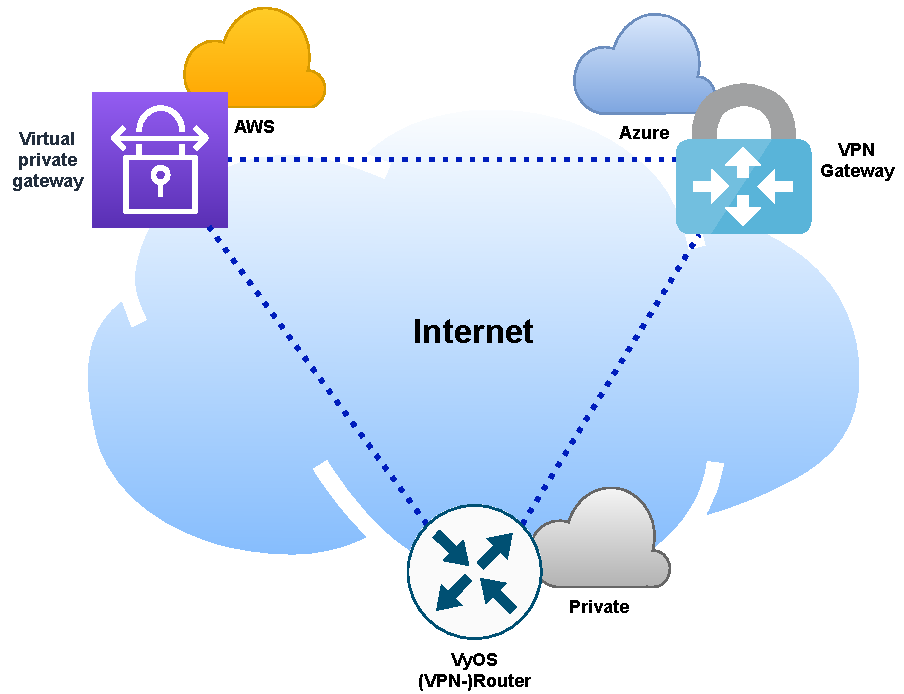
\includegraphics{Figures/Use-Case-1_Basis_Deployment.pdf}
  \caption{Basis Deployment}
  \label{grafik:Use-Case-1_Basis_Deployment}
\end{figure}


%Kein NAT, da am Anfang evtl. einfacher, aber am Ende nur Ärger und Freischaltungen etc...

%Um den Anspruch der Automatisierung gerecht zu werden, ...
\subsection{Evaluationskriterien}
Nach der Umsetzung wird evaluiert, ob das Deployment folgender Kriterien erfolgreich war:
\begin{enumerate}
    \item IPv4-Adressbereiche werden im IPAM reserviert und mit AWS VPC und Azure VNET assoziiert. Test-Szenario: Zur Verifizierung werden die reservierten Adressbereiche mit den assoziierten verglichen.
    \item IPSEC-Verbindungen werden zwischen allen VPN-Gateways aufgebaut. Test-Szenario: Dies kann mit einem Blick in die verschiedenen \textit{Dashboards} der Cloud-Plattformen bzw. CLI-Kommando (VyOS) verifiziert werden.
    %FIB in technischen Grundlagen?
    \item BGP-Sessions werden etabliert und Präfixe zwischen den Teilnehmern ausgetauscht. Die Routen müssen in der Routing-Tabelle sichtbar sein. Test-Szenario: Eine Testmaschine pro Site und Ping-Tests zwischen den Sites veranlasst werden.
    %Evtl. noch testen, ob Pings auch bei Verbindungsverlust funktionieren
    \item Die Präfixe sollten im Normalfall über verschiedene AS-Pfade sichtbar sein. Nur bei Verbindungsverlust sind Präfixe ausschließlich über einen AS-Pfad zu sehen. Tests finden analog zu Punkt 2 statt.
\end{enumerate}
\chapter{Umsetzung der Use-Cases und Evaluation} \label{Umsetzung der Use-Cases und Evaluation}

\section{Use-Case 1: Basis Deployment} \label{Use-Case 1: Basis Deployment}
%IPAM-Vorbereitungen, TF Matching erläutern
%Was ist ein Subnet im Cloud-Kontext? Einleitung?
%TF: Resource, Data, Modul, Provider
\subsection{Umsetzung: Kerntätigkeiten}

Im PHPIPAM müssen mehrere Netzbereiche reserviert werden. Es werden Netzbereiche benötigt, in denen Maschinen per IPv4 kommunizieren können. Diese Netze werden mit VPC bzw. VNET assoziiert. Für VNET wurde der Netzblock \glqq 10.32.0.0/16\grqq{} und für VPC der Netzblock \glqq 10.33.0.0/16\grqq{} vorreserviert, aus dem kleinere {Subnets} für die jeweilige Cloud entnommen werden können. Weiterhin ist die Annahme, dass die Private Cloud bereits einen Netzbereich besitzt, in dem Maschinen angesiedelt sind: \glqq 192.168.201.0/24.\grgg{}\\
%https://docs.aws.amazon.com/vpn/latest/s2svpn/VPNTunnels.html
%https://docs.microsoft.com/de-de/azure/vpn-gateway/bgp-howto
Weiterhin benötigt man {Transfernetzwerke}, über die die IPv4-Pakete geschickt werden und die BGP-Präfixe ausgetauscht werden können. AWS sieht hierfür /30-Präfixe aus dem Bereich \glqq 169.254.0.0/16\grqq{} vor, Azure hat eine Range reserviert: \glqq 169.254.21.0 - 169.254.22.255\grqq{}. Als Kompromiss können daher nur Netze aus den Azure-Bereichen genutzt werden, da die Bereiche, die AWS zur Verfügung stellt, größtenteils außerhalb dieser Range liegen. Auch diese Netzbereiche müssen im IPAM vorreserviert werden, auch die Transfernetze automatisiert ausgebracht werden.\\
Im folgenden Code-Beispiel wird innerhalb des IPAM nach dem Bereich \glqq TF\_CLOUD\_BGP\_TRANSFER\grqq{}, aus dem alle Transfernetze entommen werden, gesucht. Innerhalb des Bereichs wird aus dem vorreservierten Block \glqq Cloud\_Transfer\_BGP\_1\grqq{} ein /30-Netzwerk entnommen. Die Reservierung der Netzblöcke für VPC und VNET erfolgen analog.
%data vs. resource in Einleitung erläutern?
\begin{lstlisting}[label=network-reservation-ip,caption=Die data-Anweisungen dienen ausschließlich der Suche nach dem passenden Transfernetzwerk-Block. Per resource-Anweisung wird ein /30-Netzwerk reserviert.]
//Azure - AWS Transfer
data "phpipam_section" "apipa_main_section" {
  name = "TF_CLOUD_BGP_TRANSFER"
}
data "phpipam_subnet" "apipa_transfer_subnet" {
  section_id = data.phpipam_section.apipa_main_section.section_id
  description_match = "Cloud_Transfer_BGP_1"
} 
resource "phpipam_first_free_subnet" "free_subnet_apipa" {
  parent_subnet_id = data.phpipam_subnet.apipa_transfer_subnet.subnet_id
  subnet_mask = 30
  description = "BGP_AWS_AZURE"
}
\end{lstlisting}

Es ist auch möglich, dass IPv4-Adressen für Transfernetze automatisch von Azure bzw. AWS vorgegeben werden. Mit dem avisierten Backbone-Design aus drei Teilnehmern lässt sich das allerdings nicht vereinbaren: die Adressbereiche müssen vom IPAM vorgegeben werden (vgl. später: Probleme statische Route).\\
Weiterhin werden Pre-Shared-Keys für die Aushandlung der IPSEC-Verbindungen benötigt. AWS erzeugt automatisch solche Schlüssel, welche durch das Terraform-Modul \glqq aws\_vpn\_connection\grqq{} zurückgegeben werden. Diese automatisch erzeugten Schlüssel werden daher für die Backbone-Verbindungen AWS <-> Azure und AWS <-> Private Cloud (VyOS) genutzt. Da Azure diese Schlüssel nicht erzeugt, wurde ein Terraform-Modul geschrieben, welches diese Schlüssel aus 24 Zeichen erzeugt. Dieses kann anschließend genutzt werden für die Backbone-Verbindung Azure <-> Private Cloud (VyOS).

\begin{lstlisting}[label=tf-generate-psk,caption=Auf Sonderzeichen (special) wurde verzichtet. Das Modul stellt per output-Anweisung den Schlüssel für andere Terraform-Module zur Verfügung.]
resource "random_password" "random_password" {
  length = 24
  lower = true
  upper = true
  number = true
  special = false
}
output "azure_vyos_tunnel1_psk" {
  value = random_password.random_password.result
  sensitive = true
}
\end{lstlisting}

%alles Devices nennen?
Da, wie bereits erwähnt (vgl. klick), für die VyOS-Router keine Terraform-Integration verfügbar ist, wurde zur Konfiguration des Devices eine Vorlage erstellt.

%https://www.terraform.io/docs/language/functions/templatefile.html
Die Erzeugung der Vorlage erfolgt über die Funktion templatefile().

\begin{lstlisting}[label=tf-call-tpl-generation,caption=Die Funktion templatefile() erzeugt aus einer Template-Datei (vyos\_config.tpl) die Datei /tmp/example.sh. Die Template-Datei wird mit den Variablen var.aws\_vgw\_ip und aws\_tunnel1\_psk befüllt.]
resource "local_file" "vyos_config" {
  filename = /tmp/example.sh
  content = templatefile("${path.module}/include/vyos_config.tpl",
  {
    aws_vgw_ip = var.aws_vgw_ip
    aws_tunnel1_psk = var.aws_tunnel1_psk
    [ ... weitere Aufrufparameter ...]
  })
}
\end{lstlisting}


\begin{lstlisting}[label=tf-generate-tpl,caption=Verschiede set-Kommandos werden in ein VyOS-Skript eingebettet (Interpreter: /bin/vbash). Die Variablen in Zeilen 9-12 resultieren aus dem Funktionsaufruf (s.o.).]
$ head -n 11 < vyos/include/vyos_config.tpl
#!/bin/vbash
source /opt/vyatta/etc/functions/script-template
configure
#AWS
set vpn ipsec ike-group AWS lifetime '28800'
set vpn ipsec ike-group AWS proposal 1 dh-group '2'
set vpn ipsec ike-group AWS proposal 1 encryption 'aes128'
set vpn ipsec ike-group AWS proposal 1 hash 'sha1'
set vpn ipsec site-to-site peer ${aws_vgw_ip} authentication mode 'pre-shared-secret'
set vpn ipsec site-to-site peer ${aws_vgw_ip} authentication pre-shared-secret ${aws_tunnel1_psk}
set vpn ipsec site-to-site peer ${aws_vgw_ip} description 'VPC tunnel 1'
\end{lstlisting}

\begin{lstlisting}[label=tf-generate-psk,caption=Das so generierte Shell-Skript wird per SSH auf das Zielsystem (VyOS-Router) hochgeladen und per provisioner remote-exec ausgeführt.]
resource "null_resource" "vyos_config" {
  connection {
    type = "ssh"
    host = var.vyos_host
    user = var.ssh_user
    private_key = file(var.private_key_file)
  }
  provisioner "file" {
   source = /tmp/example.sh
   destination = var.vyos_script_path
  }
  provisioner "remote-exec" {
    inline = [ "chmod +x ${var.vyos_script_path}", var.vyos_script_path ]
  }
}
\end{lstlisting}

Nach dem erfolgreichen Deployment wird folgender Status von Terraform zurückgemeldet:
\begin{lstlisting}[label=tf-base-deployment-ok,caption=Terraform Deployment Status]
BLIBLABLUB
\end{lstlisting}

\begin{lstlisting}[label=tf-base-deployment-ipsec-ok,caption=IPSEC Status]
vyos@vyos-cloud:~$ show vpn ipsec sa
Connection                      State    Uptime    Bytes In/Out    Packets In/Out    Remote address    Remote ID    Proposal
------------------------------  -------  --------  --------------  ----------------  ----------------  -----------  ----------------------------------
peer-18.158.151.142-tunnel-vti  up       24s       1K/3K           19/44             18.158.151.142    N/A          AES_CBC_128/HMAC_SHA1_96/MODP_1024
peer-20.67.177.217-tunnel-vti   up       24s       652B/223B       4/3               20.67.177.217     N/A          AES_CBC_256/HMAC_SHA1_96
peer-20.67.177.217-tunnel-vti   up       24s       1K/132B         17/3              20.67.177.217     N/A          AES_CBC_256/HMAC_SHA1_96/MODP_1024
\end{lstlisting}


Außerdem wurden auf dem Cloud-Router die AWS- und Azure-Präfixe via BGP installiert. Pro Präfix sind zwei Pfade vorhanden:

\begin{lstlisting}[label=tf-base-deployment-bgp-ok,caption=BGP Status]
vyos@vyos-cloud:~$ sh ip bgp | grep -A1 -E '10.3[2|3]'
*  10.32.0.0/16     169.254.53.1           100             0 65516 65515 i
*>                  169.254.21.6                           0 65515 i
*  10.33.0.0/24     169.254.21.6                           0 65515 65516 i
*>                  169.254.53.1           100             0 65516 i
\end{lstlisting}

Hier sind auch die ersten Unterschiede zwischen den beiden Cloud-Plattformen zu erkennen: Während AWS den kompletten VPC CIDR-Block per BGP bekannt macht (/16), passiert das bei Azure nur für die Subnets, die dem VNET Address space entnommen wurden.
%Probleme: Race Condition externe IP, Redeploy wegen TF Bug, statische Route zu BGP Neighbor (Azure - AWS: Pseudo directly, Azure - VyOS: Static, Azure - AWS), stateless VyOS Config
\subsection{Probleme und Lösungsfindung}

%Härtung IPSEC Parameter? GCM usw...

\section{Use-Case 2: Road Warrior} \label{Use-Case 2: Road Warrior}

\section{Use-Case 3: Server-zu-Server} \label{Use-Case 3: Server-zu-Server}


%\include{Chapters/05_Evaluation}
%\include{Chapters/06_Fazit_und_Ausblick}
\chapter{Example}
\label{ch:example}

!!! Please delete this chapter after finishing your work !!!

\section{Settings}

To add your name and the title of your work, please use the ``Settings.tex'' file!
Additionally, switch there between German and English version.

\section{How to Make Sections and Subsections}

Use section and subsection commands to organize your document. \LaTeX{} handles all the formatting and numbering automatically. Use ref and label commands for cross-references.

\subsection{How to Make Lists}

You can make lists with automatic numbering \dots

\begin{enumerate}
\item Like this,
\item and like this.
\end{enumerate}
\dots or bullet points \dots
\begin{itemize}
\item Like this,
\item and like this.
\end{itemize}
\dots or with words and descriptions \dots
\begin{description}
\item[Word] Definition
\item[Concept] Explanation
\item[Idea] Text
\end{description}

\section{Section}

You have to write text between each headline.

\section{Citation}

This part describes the three types of citations which are possible:

\section{Direct Citation}

The maximum for a direct citation is a ${1/2}$ page.

\begin{quotation}
	Overview first, zoom and filter, then details-on-demand
	\autocite{shneiderman_eyes_1996}
\end{quotation}

\section{Floating Text Citation}

\textcite{shneiderman_eyes_1996} defined the Visual Information Seeking Mantra as ``Overview first, zoom and filter, then details-on-demand''.

\section{Indirect Citation}

Some text which summarizes a paper or a book chapter. This could take several lines.
Find attached a citation of a website~\autocite{kaley_match_2018}.

\newpage
\section{Figures}

To place a figure use the following code example

\begin{figure}[ht!]
  \centering
  \includegraphics[width=1\columnwidth]{Figures/Example}
  \caption{Interactive data exploration with multiple devices.}
  \label{fig:example}
\end{figure}




\begin{figure}[h]
    \centering
    \subfigure[Figure A]{
    	\label{fig:a}
        \includegraphics[width=60mm]{Figures/Example}
     }
	\subfigure[Figure B]{
    	\label{fig:b}
        \includegraphics[width=60mm]{Figures/Example}
     }
    \caption{Wearables worn for experiments 1, 2, and 3.}\label{fig:figure2}
\end{figure}

Refer to a figure in the following forms:\\
If you take a look at Figure~\ref{fig:example} ...\\
... text text (see Figure~\ref{fig:example}) ...

\section{Listings}
\begin{lstlisting}[caption=A bit of source code., label=lst:test]
if( true == questions )
{
    std::cout << "Let me google it for you";
}
else
{
    std::cout << "Great";
}
\end{lstlisting}

Now lets take a look at Listing~\ref{lst:test}.


\section{Table}

\begin{table}[ht!]
  \caption{My caption with a very useful description. die kann auch etwas länger sein und über mehrere Zeilen gehen und so weiter.}
  \label{my-label}
  \begin{tabular}{llr}
    \hline
    \multicolumn{2}{c}{Item} &            \\ \cline{1-2}
    Animal     & Description & Price (\$) \\ \hline
    Gnat       & per gram    & 13.65      \\
               & each        & 0.01       \\
    Gnu        & stuffed     & 92.50      \\
    Emu        & stuffed     & 33.33      \\
    Armadillo  & frozen      & 8.99       \\ \hline
  \end{tabular}
\end{table}

For the fast generation of tables from Excel use \url{http://www.heise.de/download/excel2latex.html}

\section{Equations}

\LaTeX{} is great at typesetting equations. Let $X_1, X_2, \ldots, X_n$ be a sequence of independent and identically distributed random variables with $\text{E}[X_i] = \mu$ and $\text{Var}[X_i] = \sigma^2 < \infty$, and let

$$S_n = \frac{X_1 + X_2 + \cdots + X_n}{n}$$

This was a equation without a label.
      
\begin{equation}
S_n = \frac{1}{n}\sum_{i}^{n} X_i
\label{eq:test}
\end{equation}

This is the reference to equation~\ref{eq:test}.      

denote their mean. Then as $n$ approaches infinity, the random variables $\sqrt{n}(S_n - \mu)$ converge in distribution to a normal $\mathcal{N}(0, \sigma^2)$.



\pagestyle{plain} 

%Literaturverzeichnis
\newpage
\bibliographystyle{unsrt}
\bibliography{biblatex}

\listoffigures

\end{document}























